\documentclass[a4paper,11pt]{article}

\usepackage[T1]{fontenc}
\usepackage[utf8]{inputenc}
\usepackage{graphicx}
\usepackage{xcolor}

\renewcommand\familydefault{\sfdefault}
\usepackage{tgheros}

\usepackage{amsmath,amssymb,amsthm,textcomp}
\usepackage{enumerate}
\usepackage{multicol}
\usepackage{tikz}
\usepackage{pdfpages}
\usepackage{hyperref}


\graphicspath{ {.} }
\usepackage{geometry}
\geometry{left=25mm,right=25mm,%
bindingoffset=0mm, top=20mm,bottom=20mm}



\usepackage{tabularx,lipsum,environ,amsmath,amssymb}

\makeatletter
\newcommand{\problemtitle}[1]{\gdef\@problemtitle{#1}}% Store problem title
\newcommand{\problemquestion}[1]{\gdef\@problemquestion{#1}}% Store problem question
\newcommand{\problemsolution}[1]{\gdef\@problemsolution{#1}}% Store problem input
\NewEnviron{problem}{
  \problemtitle{}\problemquestion{}\problemsolution{}% Default input is empty
  \BODY% Parse input
  \par\addvspace{.5\baselineskip}
  \noindent
  \begin{tabularx}{\textwidth}{@{\hspace{\parindent}} l X c}
    \multicolumn{2}{@{\hspace{\parindent}}l}{\@problemtitle} \\% Title
    \textbf{Description:} & \@problemquestion \\% Question
        \textbf{Solution:} & \@problemsolution % Input
  \end{tabularx}
  \par\addvspace{.5\baselineskip}
}
\makeatother



\linespread{1.3}

\newcommand{\linia}{\rule{\linewidth}{0.5pt}}

% custom theorems if needed
\newtheoremstyle{mytheor}
    {1ex}{1ex}{\normalfont}{0pt}{\scshape}{.}{1ex}
    {{\thmname{#1 }}{\thmnumber{#2}}{\thmnote{ (#3)}}}

\theoremstyle{mytheor}
\newtheorem{defi}{Definition}

% my own titles
\makeatletter
\renewcommand{\maketitle}{
\begin{center}
\vspace{2ex}
{\huge \textsc{\@title}}
\vspace{1ex}
\\
\linia\\
\@author \hspace{100ex} m.plevako@innopolis.university \hspace{100ex} BS18-02 \hspace{100ex} Variant (c)

\vspace{4ex}
\end{center}
}
\makeatother
%%%

% custom footers and headers
\usepackage{fancyhdr}
\pagestyle{fancy}
\lhead{}
\chead{}
\rhead{}
\lfoot{Assignment \textnumero{} 5}
\cfoot{}
\rfoot{Page \thepage}
\renewcommand{\headrulewidth}{0pt}
\renewcommand{\footrulewidth}{0pt}
% 

% code listing settings
\usepackage{listings}
\lstset{
    language=Python,
    basicstyle=\ttfamily\small,
    aboveskip={1.0\baselineskip},
    belowskip={1.0\baselineskip},
    columns=fixed,
    extendedchars=true,
    breaklines=true,
    tabsize=4,
    prebreak=\raisebox{0ex}[0ex][0ex]{\ensuremath{\hookleftarrow}},
    frame=lines,
    showtabs=false,
    showspaces=false,
    showstringspaces=false,
    keywordstyle=\color[rgb]{0.627,0.126,0.941},
    commentstyle=\color[rgb]{0.133,0.545,0.133},
    stringstyle=\color[rgb]{01,0,0},
    numbers=left,
    numberstyle=\small,
    stepnumber=1,
    numbersep=10pt,
    captionpos=t,
    escapeinside={\%*}{*)}
}

%%%----------%%%----------%%%----------%%%----------%%%

\begin{document}

\title{HW \textnumero{} 5}

\author{Matvey Plevako}

\maketitle


\section*{Problem}

% 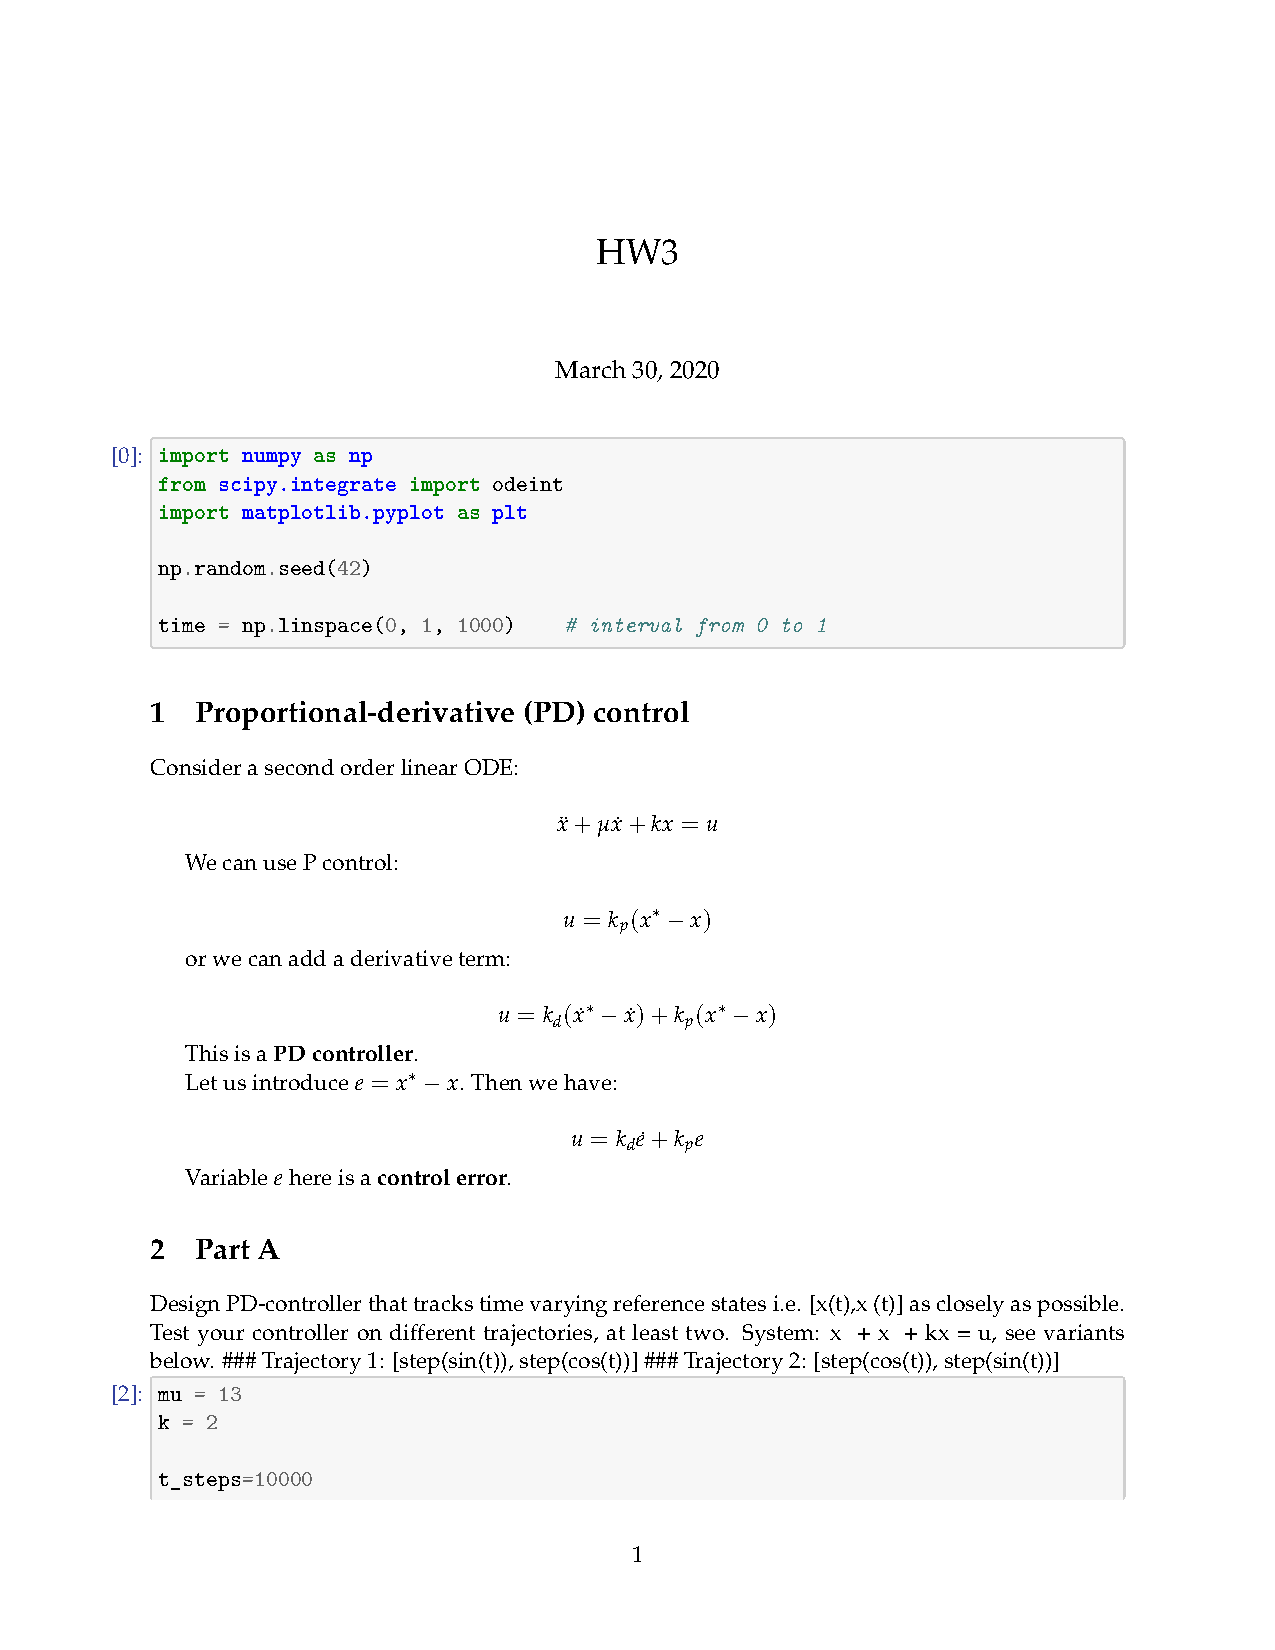
\includepdf[pages=-]{HW3_task1.pdf}


\section*{Problem 1}
Consider classical benchmark system in control theory - inverted pendulum on a cart (Figure 1). It is nonlinear under-actuated system that has the following dynamics.
  $$(M + m)\ddot{x} - ml \cos(\theta) \ddot{\theta}+ ml \sin(\theta) \dot{\theta}^2 = F$$
$$- \cos(\theta)\ddot{x} + l\ddot{\theta}- g \sin(\theta) = 0$$
\begin{center}
    where $g = 9.81$ is gravitational acceleration.
    $$(c)M = 3.6,m = 3.6,l = 1.01$$
The system dynamics can be written in state space form:
$$\dot{z} = f (z) + g(z)u$$
$$y = h(z) = \begin{bmatrix}x & \theta\end{bmatrix}^T$$

where $z =  \begin{bmatrix}x & \theta & \dot{x} & \dot{\theta}\end{bmatrix}^T$
is the state vector of the system, y is the output vector. The dynamics of the system around unstable equilibrium of the pendulum $(\bar{z} = \begin{bmatrix} 0 & 0 & 0 & 0 \end{bmatrix}^T)$ can be described by a linear system that is obtained from linearization of the nonlinear dynamics around $ \bar{z} $.

$$\delta \dot{z} = A\delta z + B\delta u$$
$$\delta y = C\delta z$$
    $$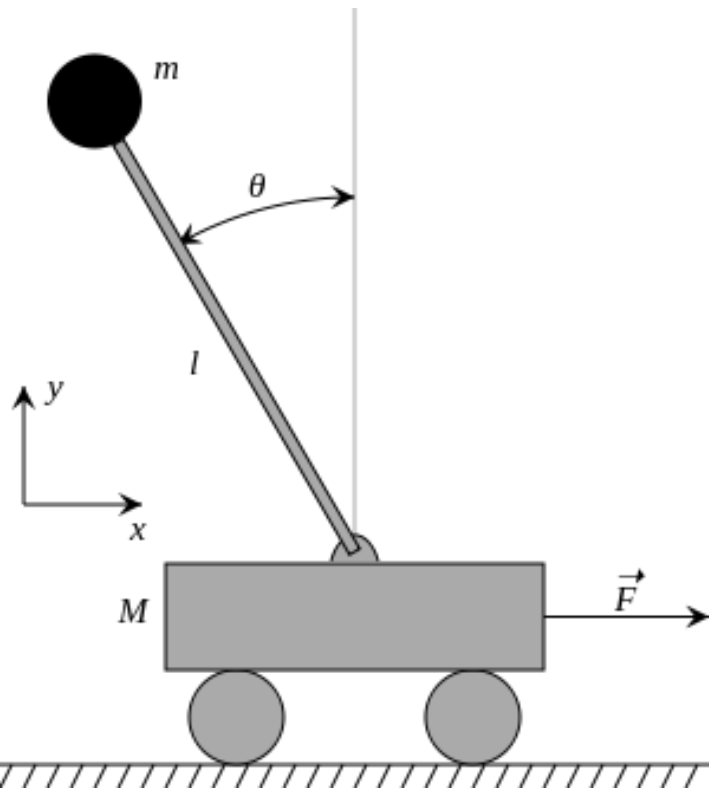
\includegraphics[width=10cm, height=10cm]{scheme.png}$$
    Figure 1: A schematic drawing of the inverted pendulum on a cart. The rod is considered massless. The mass of the cart and the point mass at the end of the rod are denoted by M and m. The rod has a length l.
\end{center}



\section*{part A}
\begin{problem}
  \problemquestion{prove that it is possible to design state observer of the linearized system}
  \problemsolution{
System is observable, if matrix $S = \begin{bmatrix} C \\ CA \\ CA^2 \\ CA^3\end{bmatrix}$ has rank 4
$$C = \begin{bmatrix} 1 & 0 & 0 & 0 \\ 0 & 1 & 0 & 0 \end{bmatrix}$$

$$CA = \begin{bmatrix} 0 & 0 & 1 & 0 \\ 0 & 0 & 0 & 1 \end{bmatrix}$$

$$CA^2 = \begin{bmatrix} 0 & \frac{mg}{M} & 0 & 0 \\ 0 & \frac{g(m+M)}{lM} & 0 & 0 \end{bmatrix}$$

$$CA^3 = \begin{bmatrix} 0 & 0 & 0 & \frac{mg}{M} \\ 0 & 0 & 0 & \frac{g(m+M)}{lM}\end{bmatrix}$$
$$S = \begin{bmatrix} 1 & 0 & 0 & 0 \\ 0 & 1 & 0 & 0 \\ 0 & 0 & 1 & 0 \\ 0 & 0 & 0 & 1 \\ 0 & \frac{mg}{M} & 0 & 0 \\ 0 & \frac{g(m+M)}{lM} & 0 & 0 \\ 0 & 0 & 0 & \frac{mg}{M} \\ 0 & 0 & 0 & \frac{g(m+M)}{lM} \end{bmatrix}$$
We can see the Identity matrix 4x4 at the upper part of the S matrix => its rank is 4
  }
\end{problem}


\section*{part B}
\begin{problem}
  \problemquestion{for open loop state observer, is the error dynamics stable?}
  \problemsolution{Open-loop state observer has a form: $\hat{\dot{z}} = A\hat{z} + Bu$
  Error dynamics:
    
$\epsilon = \hat{z} - z$, $\dot{z} = Az + Bu$ , $\dot{\epsilon} = A \epsilon $

Thus, open loop state observe is stable, when A is negative definite, which is not the case, becaue:

$Det (\begin{bmatrix} -\lambda & 0 & 1 \\ 0 & -\lambda & 0 & 1 \\ 0 & \frac{mg}{M} & -\lambda & 0 \\ 0 & \frac{g(M+m)}{lM} & 0 & -\lambda \end{bmatrix}) = -\lambda(-\lambda^3 + \lambda(\frac{g(M+m)}{lM})) = \lambda^2(\lambda^2 - \frac{g(M+m)}{lM})$ if $\lambda = 0 $ or $\lambda = \pm \sqrt{\frac{g(M+m)}{lM}}$ $\lambda = \pm 4,4052174287$}
\end{problem}

\section*{part C}
\begin{problem}
  \problemquestion{design Luenberger observer for linearized system using both pole placement and LQR methods}
  \problemsolution{Luenberger observer has form: 
$$\hat{\dot{z}}_{k+1} = A\hat{z_k} + Bu_k + L (y_k - \hat{y_k})$$
$$\hat{y_k} = C\hat{z_k} + Du_k$$
In the given case, $D = 0$
Pole placement method:

it is usually used in case: $A - BL \prec 0 $, 

now the system $A - LC \prec  0 $ is given, if it is transposed: $A^T-C^TL^T \prec 0 $ 
$$L^T = poles(A^T, C^T, eigVals)$$

LQR method (possible, because, C is a part of Identity matrix):

$$L^T = lqr(A^T, C^T, Q, R)$$
}
\end{problem}

\begin{lstlisting}[label={list:first}]
import numpy as np
import matplotlib.pyplot as plt
import scipy.signal as sig
from scipy.integrate import odeint
import scipy.linalg as lin

g = 9.81
M = 3.6
m = 3.6
l = 1.01

eig = [-1.1, -1.2, -1.3, -1.4]

A = np.array([[0, 0, 1, 0], [0, 0, 0, 1], [0, g*m/M, 0, 0], [0, g*(M+m)/l/M, 0, 0]])
B = np.array([0, 0, 1/M, 1/l/M]).reshape(1, -1).T
C = np.array([[1, 0, 0, 0], [0, 1, 0, 0]])
#  pole placement method
pole = sig.place_poles(A.T, C.T, eig)
L_pole = pole.gain_matrix.T

# lqr method
# Q, R - random, but appropriate
Q = np.array([[1, 0, 0, 0], 
              [0, 1, 0, 0], 
              [0, 0, 1, 0], 
              [0, 0, 0, 1]])

R = np.array([[4, 1], [1, 4]]) 

S = lin.solve_continuous_are(A.T, C.T, Q, R)
L_lqr = np.array(np.linalg.inv(R)).dot(C).dot(S).T

pole = sig.place_poles(A, B, eig)
P = -pole.gain_matrix

def usual(x, t, u):
    n = np.dot(A, x) + np.dot(B, u)
    return  n

def observer(x_hat, t, u, x):
    return np.dot(A, x_hat) + np.dot(B, u) + np.dot(L_lqr, C).dot(x - x_hat)

dt = 1/10000
T = 20
time = np.linspace(0, T, dt**(-1))

x = [np.array([0.01, 0.001, 0.01, 0.01])]
x_hat = [np.array([0.02, 0.002, 0.02, 0.02])/4]

for i in range(1, len(time)):
#     Use odeint between two dots,
#     but u is fixed between two poins
#     P controller u = Px
    local_time = np.linspace(time[i-1], time[i])
    u = np.dot(P, x[-1])

    x_dot = odeint(usual, x[-1], local_time, args=tuple([u]))
    x.append(x_dot[-1])
    
    x_hat_dot = odeint(observer, x_hat[-1], local_time, args=tuple([u, x[-1]]))
    x_hat.append(x_hat_dot[-1])

def plot_sim(x, x_hat, time):
    x = np.array(x)
    y = np.dot(C, x.T)
    x_hat = np.array(x_hat)
    y_hat = np.dot(C, x_hat.T)

    plt.figure(figsize=(8, 8))
    plt.title("Inverted pendulum system simulation")
    plt.plot(time, y[0], label="init velocity")
    plt.plot(time, y[1], label="init coordinate")

    plt.plot(time, y_hat[0], label="obs velocity")
    plt.plot(time, y_hat[1], label="obs coordinate")
    plt.grid()
    plt.legend()

plot_sim(x, x_hat, time)
\end{lstlisting}

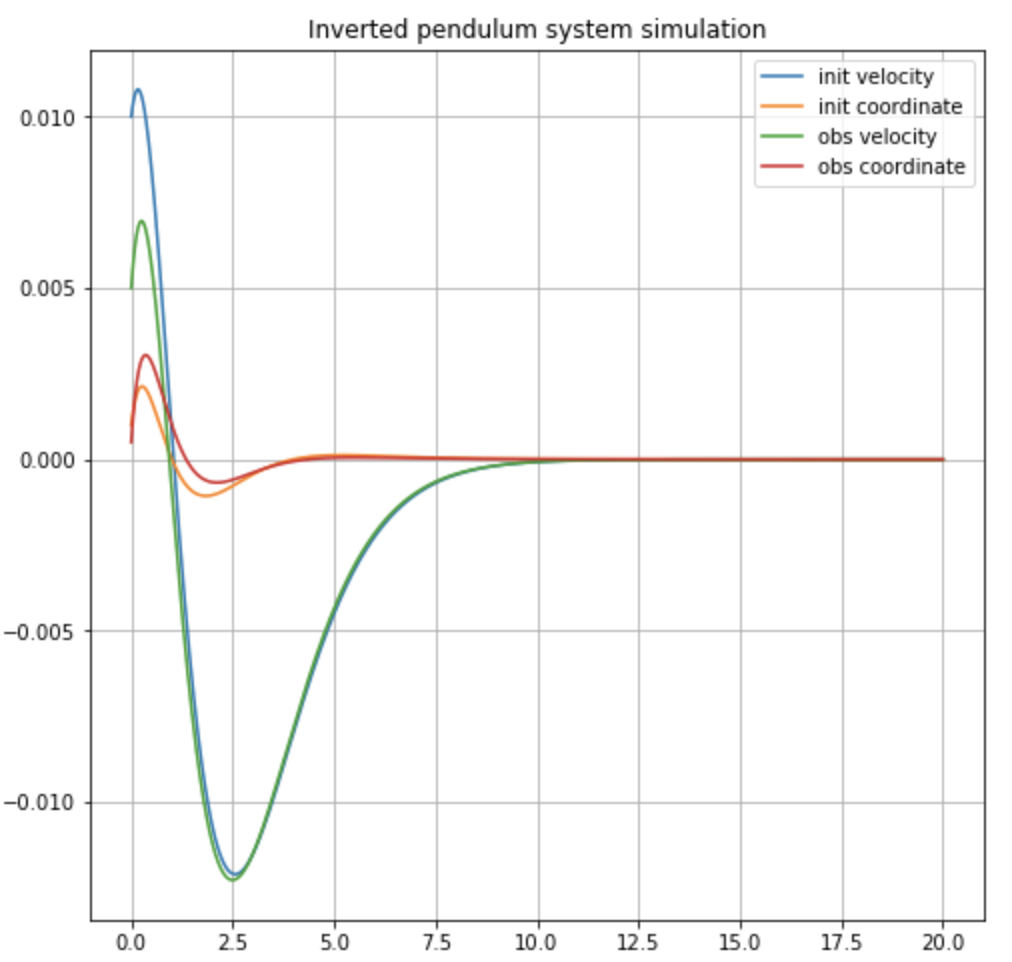
\includegraphics[width=10cm, height=9cm]{C.png}

\section*{part D}
\begin{problem}
  \problemquestion{design state feedback controller for linearized system}
  \problemsolution{}
\end{problem}
\begin{lstlisting}[label={list:second}]
res_pole = sig.place_poles(A, B, eig)
K = res_pole.gain_matrix

# visualization
def control(x, t):
    return np.dot(A - np.dot(B, K), x)

time = np.linspace(0, 20, 1000)   
x0 = x[0]
res = odeint(control, x0, time).T

fig = plt.figure(figsize=(8, 8))
plt.title("Stabilisation of the system")
plt.xlabel("time")
plt.plot(time, res[0], "r-", label="x")
plt.plot(time, res[1], "b-", label="$\theta$")
plt.plot(time, res[2], "k-", label="$\dot{x}$")
plt.plot(time, res[3], "g-", label="$\dot{\theta}$")
plt.grid()
plt.legend(shadow=True)
plt.show()
\end{lstlisting}{}

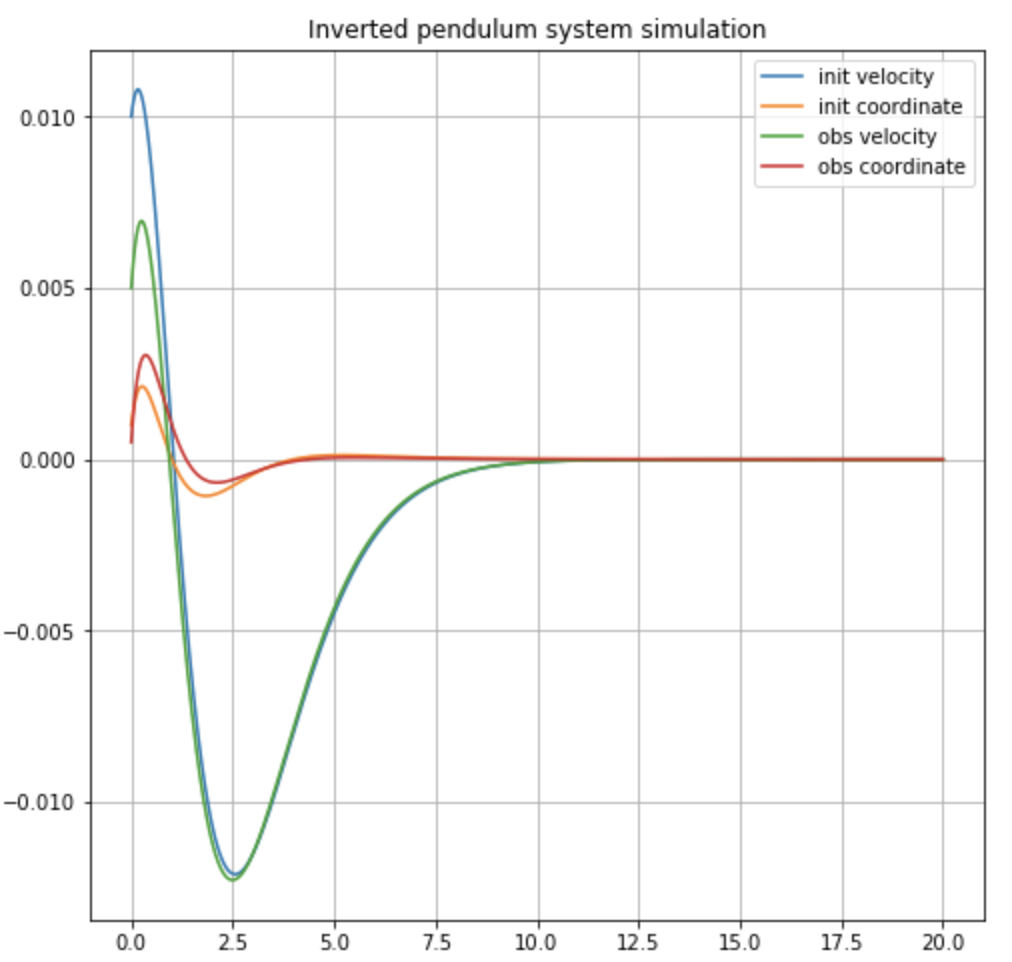
\includegraphics[width=10cm, height=9cm]{C.png}


\section*{part E}
\begin{problem}
  \problemquestion{Simulate nonlinear system with Luenberger observer and state feedback controller that uses estimated states ($u = K \hat{x}$). Make sure that the system is stabilized for various initial conditions around $\bar{z}$..}
  \problemsolution{}
\end{problem}

\begin{lstlisting}
import numpy as np
import matplotlib.pyplot as plt
import scipy.signal as sig
from scipy.integrate import odeint
import scipy.linalg as lin

g = 9.81
M = 3.6
m = 3.6
l = 1.01

eig = [-1.1, -1.2, -1.3, -1.4]

A = np.array([[0, 0, 1, 0], [0, 0, 0, 1], [0, g*m/M, 0, 0], [0, g*(M+m)/l/M, 0, 0]])
B = np.array([0, 0, 1/M, 1/l/M]).reshape(1, -1).T
C = np.array([[1, 0, 0, 0], [0, 1, 0, 0]])
#  pole placement method
pole = sig.place_poles(A.T, C.T, eig)
L_pole = pole.gain_matrix.T

# lqr method
# Q, R - random, but appropriate
Q = np.array([[1, 0, 0, 0], 
              [0, 1, 0, 0], 
              [0, 0, 1, 0], 
              [0, 0, 0, 1]])

R = np.array([[4, 1], [1, 4]]) 

S = lin.solve_continuous_are(A.T, C.T, Q, R)
L_lqr = np.array(np.linalg.inv(R)).dot(C).dot(S).T


def usual(x, t, u):
    n = np.dot(A, x) + np.dot(B, u)
    return  n


def observer(x_hat, t, u, x):
#     TRY WITH BOTH: L_lqr and L_pole
    return np.dot(A, x_hat) + np.dot(B, u) + np.dot(L_lqr, C).dot(x - x_hat)

dt = 1/10000
T = 20
time = np.linspace(0, T, dt**(-1))

x = [np.array([0.01, 0.001, 0.01, 0.01])]
x_hat = [np.array([0.02, 0.002, 0.02, 0.02])/4]

for i in range(1, len(time)):
#     Use odeint between two dots,
#     but u is fixed between two poins
#     P controller u = Px
    local_time = np.linspace(time[i-1], time[i])
    u = np.dot(P, x[-1])

    x_dot = odeint(usual, x[-1], local_time, args=tuple([u]))
    x.append(x_dot[-1])
    
    x_hat_dot = odeint(observer, x_hat[-1], local_time, args=tuple([u, x[-1]]))
    x_hat.append(x_hat_dot[-1])

plot_sim(x, x_hat, time)

\end{lstlisting}

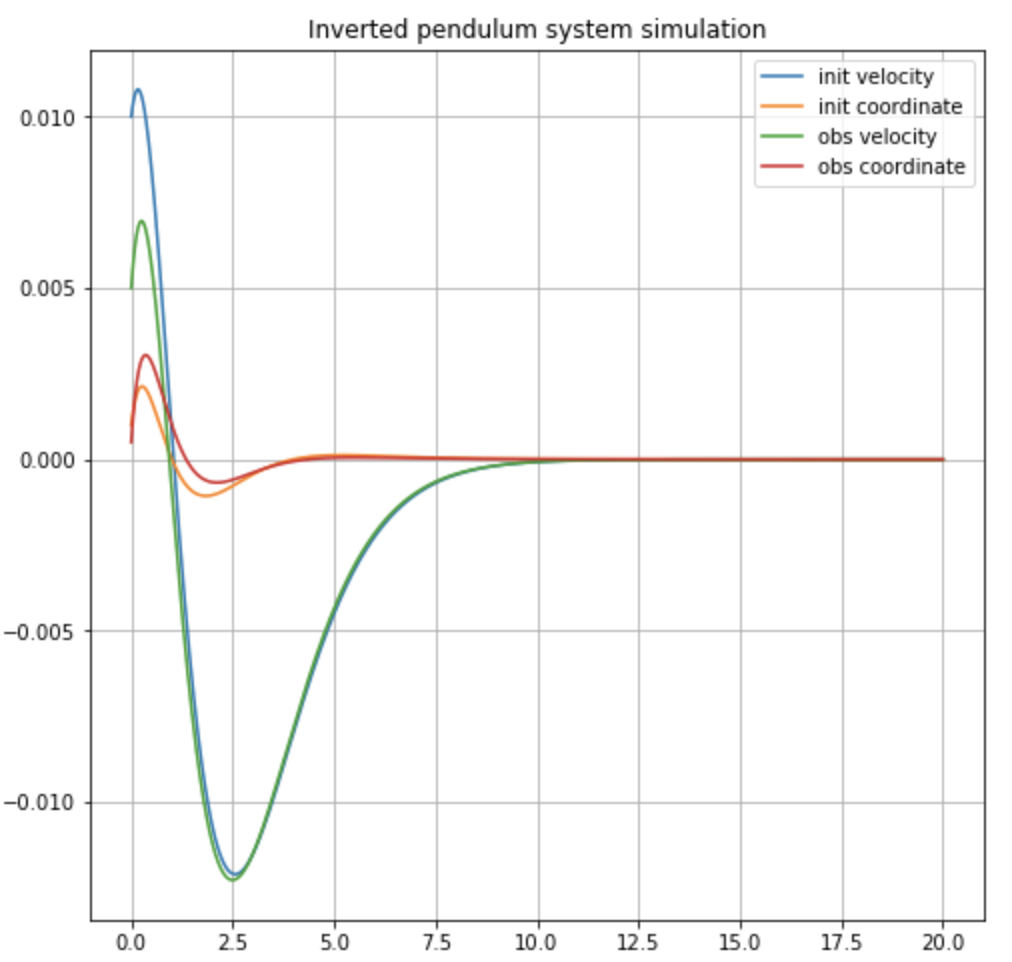
\includegraphics[width=10cm, height=9cm]{C.png}


\section*{part F}
\begin{problem}
  \problemquestion{Add white gaussian noise to the output ($\delta y = C\delta z + v$).}
  \problemsolution{}
\end{problem}


\begin{lstlisting}
def usual(x, t, u):
    n = np.dot(A, x) + np.dot(B, u)
    return  n


def observer(x_hat, t, u, dy):
    return np.dot(A, x_hat) + np.dot(B, u) + np.dot(L_lqr, dy - np.dot(C, x_hat))

dt = 1/10000
T = 20
time = np.linspace(0, T, dt**(-1))

x = [np.array([0.01, 0.001, 0.01, 0.01])]
x_hat = [np.array([0.02, 0.002, 0.02, 0.02])/4]


for i in range(1, len(time)):
#     BUT u is fixed between two poins
#     P controller u = P
    local_time = np.linspace(time[i-1], time[i])
    u = np.dot(P, x[-1])

    x_dot = odeint(usual, x[-1], local_time, args=tuple([u]))
    x.append(x_dot[-1])
    
    dy = np.dot(C, x[-1]) 
    dy += np.random.random(2) * 0.0005
    x_hat_dot = odeint(observer, x_hat[-1], local_time, args=tuple([u, dy]))
    x_hat.append(x_hat_dot[-1])

plot_sim(x, x_hat, time)
plt.show()
\end{lstlisting}

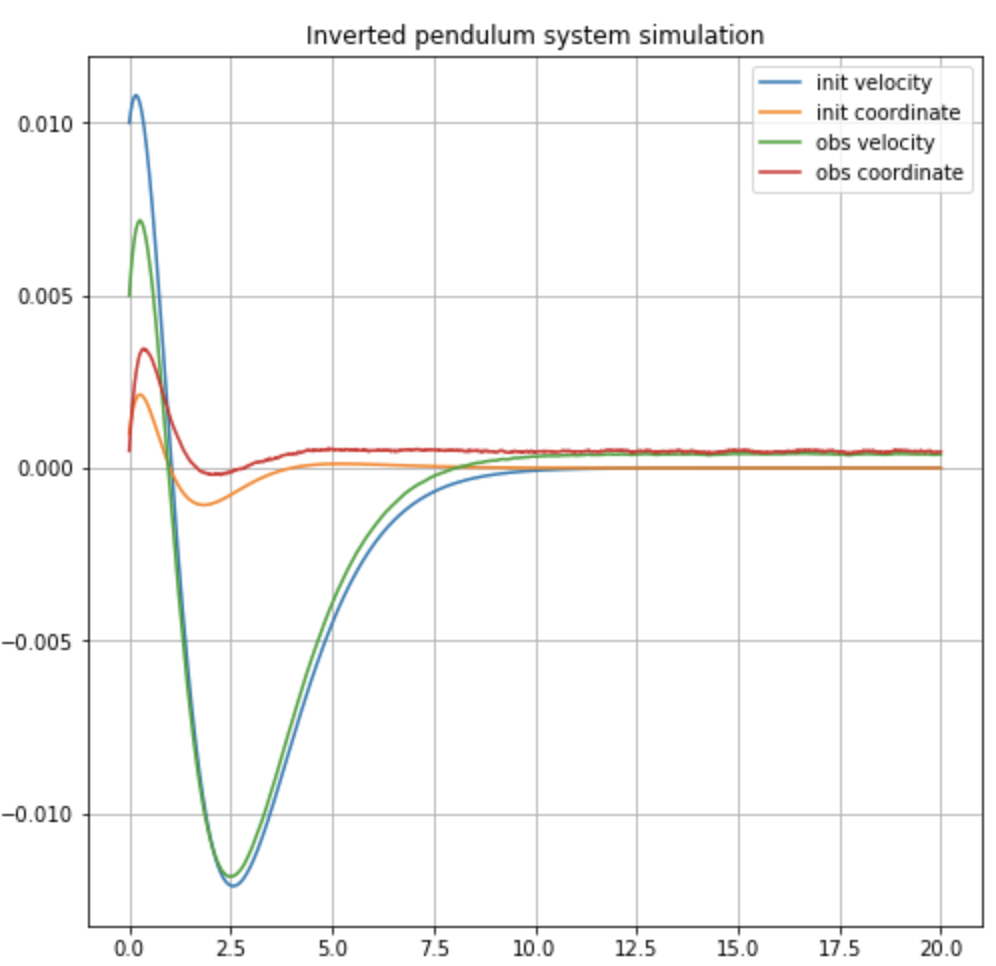
\includegraphics[width=10cm, height=10cm]{F.png}



\section*{part G}
\begin{problem}
  \problemquestion{Add white gaussian noise to the dynamics ($\delta \dot{z} = A\delta z + B\delta u + w$). What happens to the state estimation and control system?}
\end{problem}

\begin{lstlisting}
def usual(x, t, u):
    n = np.dot(A, x) + np.dot(B, u) + np.random.random(4) * 0.00005
    return  n


def observer(x_hat, t, u, dy):
    return np.dot(A, x_hat) + np.dot(B, u) + np.dot(L_lqr, dy - np.dot(C, x_hat))

dt = 1/10000
T = 20
time = np.linspace(0, T, dt**(-1))

x = [np.array([0.01, 0.001, 0.01, 0.01])]
x_hat = [np.array([0.02, 0.002, 0.02, 0.02])/4]


for i in range(1, len(time)):
#     use odeint between two dots,
#     but u is fixed between two poins
#     P controller u = Px
    local_time = np.linspace(time[i-1], time[i])
    u = np.dot(P, x[-1])

    x_dot = odeint(usual, x[-1], local_time, args=tuple([u]))
    x.append(x_dot[-1])
    
    dy = np.dot(C, x[-1]) 
    dy += np.random.random(2) * 0.0005
    x_hat_dot = odeint(observer, x_hat[-1], local_time, args=tuple([u, dy]))
    x_hat.append(x_hat_dot[-1])
    
plot_sim(x, x_hat, time)
plt.show()

\end{lstlisting}

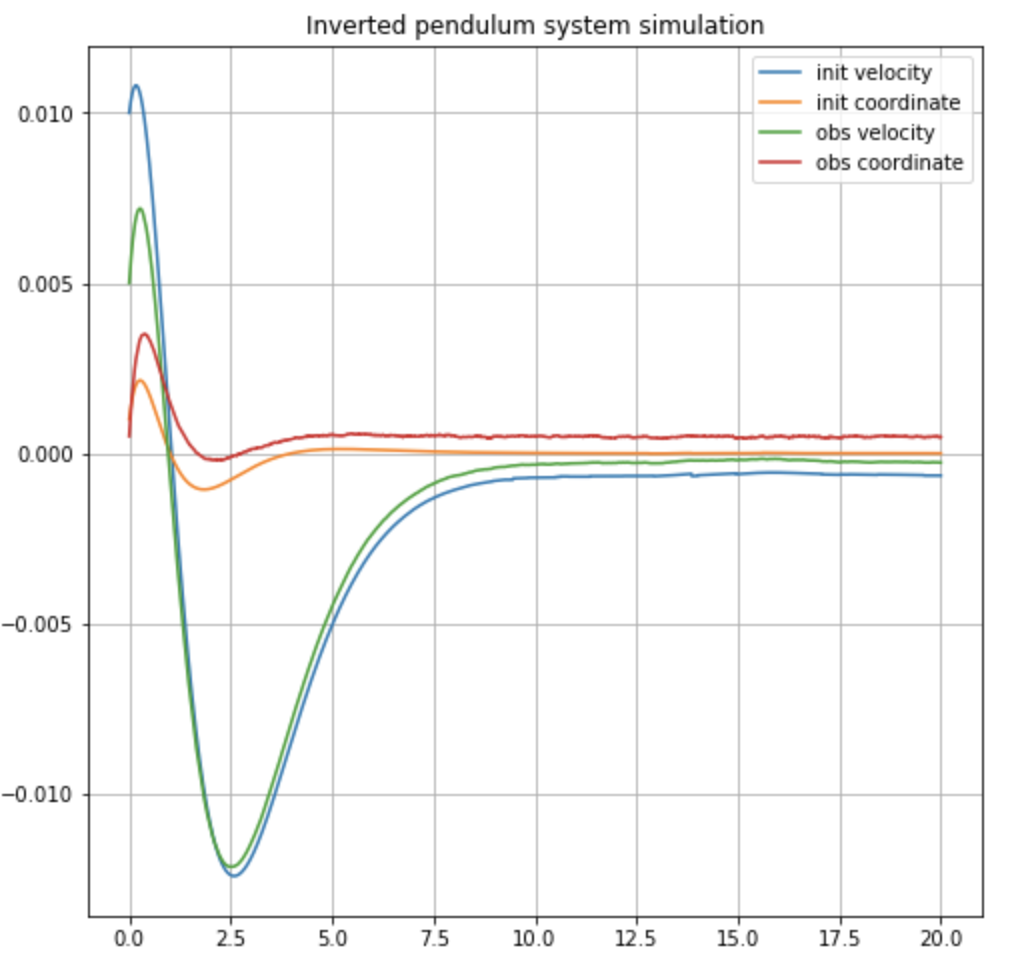
\includegraphics[width=10cm, height=10cm]{G.png}



\begin{problem}
  \problemquestion{What happens to the state estimation and control system?}
  \problemsolution{If we crop section from 12 to 14 we can see that noise does not allow to converge to 0, but it almost does not affect time to converge to "near zero" values it is 10.0 for both plots}
\end{problem}
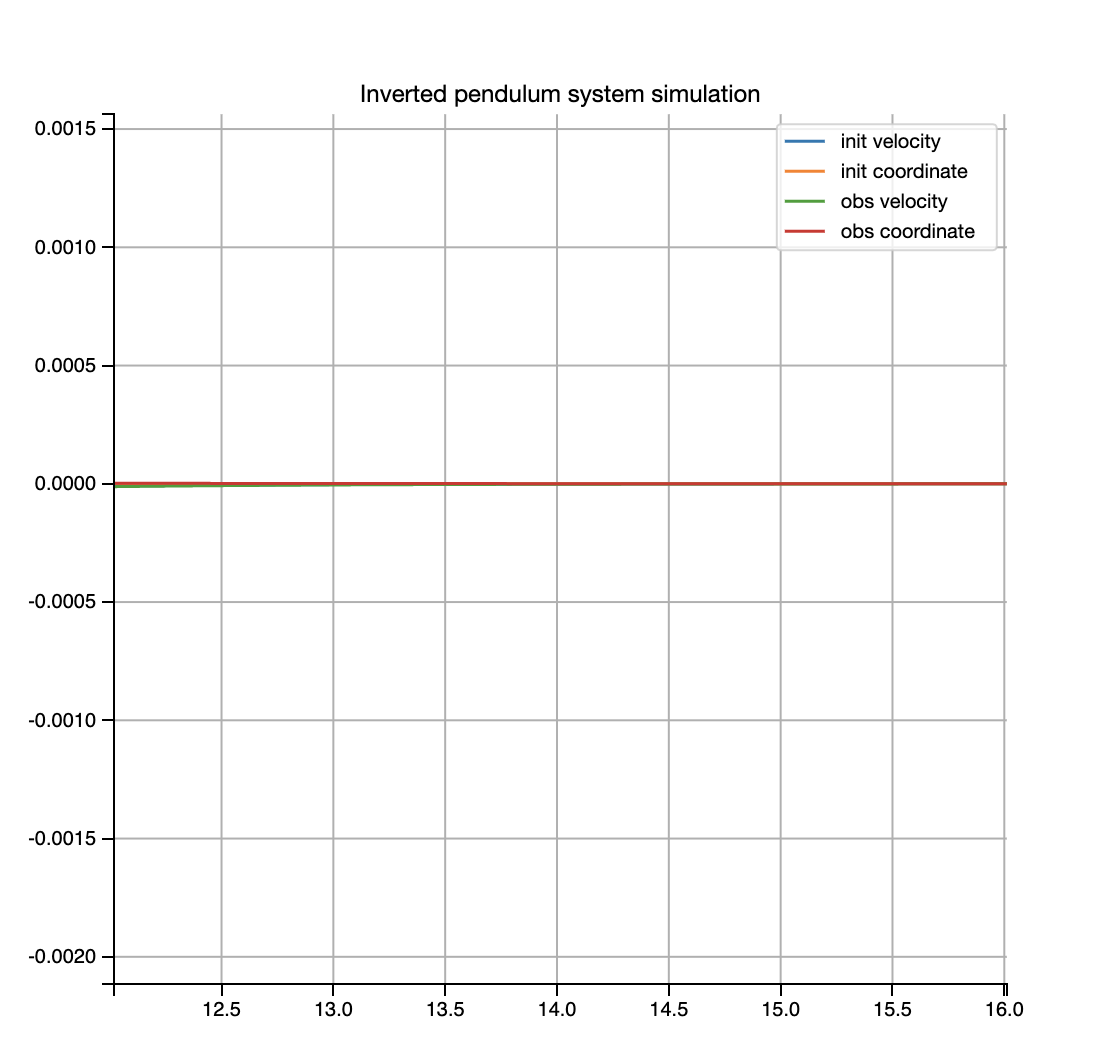
\includegraphics[width=10cm, height=10cm]{G_1.png}

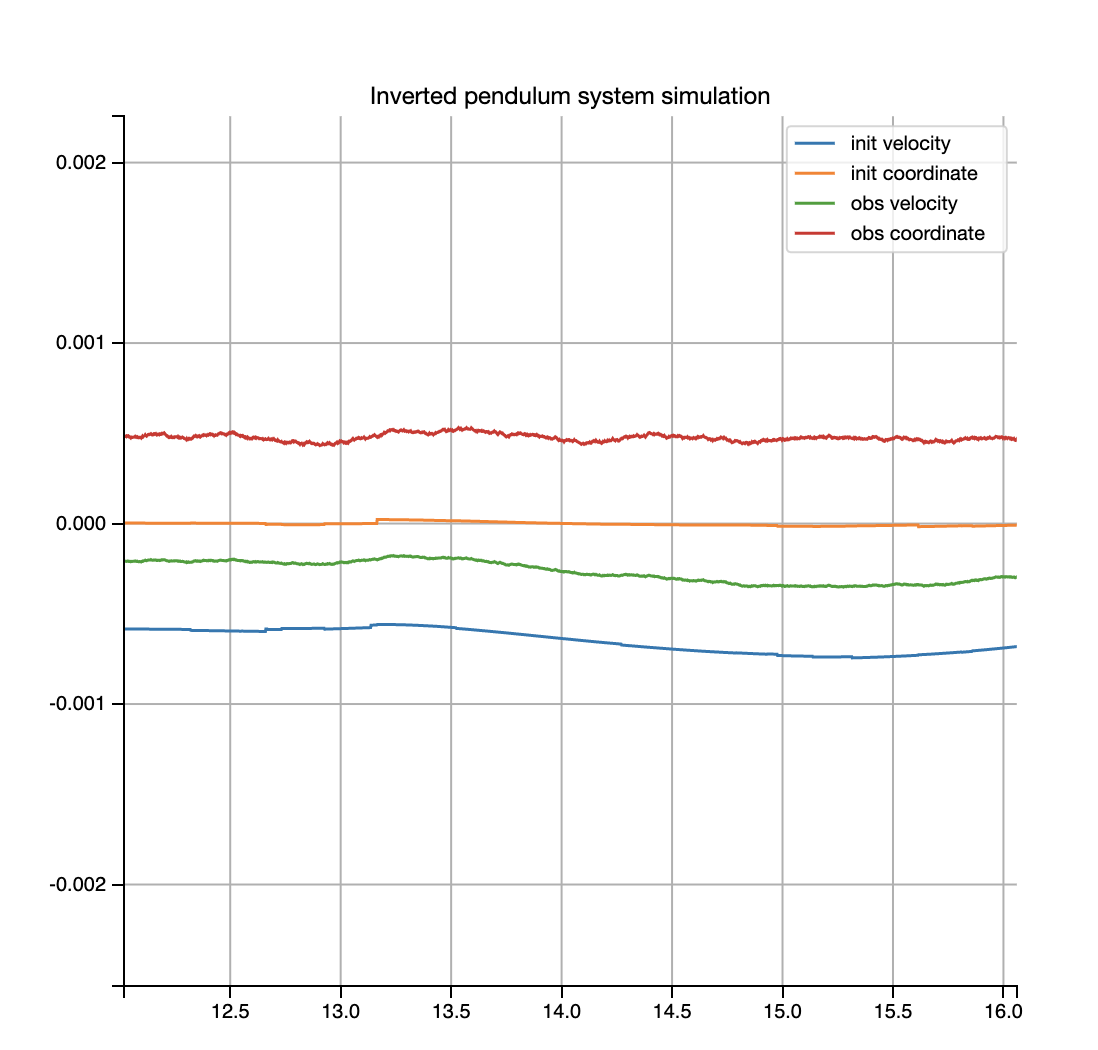
\includegraphics[width=10cm, height=10cm]{G_2.png}




\section*{part H}
\begin{problem}
  \problemquestion{implement Kalman Filter}
  \problemsolution{Prediction
  $$X^-_k = A_{k-1}X_{k-1}+B_kU_k$$
  $$P^-_k = A_{k-1}P_{k-1}A^T_{k-1}+Q_{k-1}$$
  Update
  $$V_k = Y_k-H_kX^-_k$$
  $$S_k = H_kP^-_kH^T_k+Q_{k-1}$$
  $$K_k = P^-_k H^T_kS^{-1}_k$$
  $$X_k = X^-_k + K_kV_k$$
  $$P_k = P^-_k + K_kS_kK^T_k$$
  }
\end{problem}

\begin{lstlisting}
class KalmanFilter(object):
    def __init__(self, F = None, B = None, H = None, Q = None, R = None, P = None, x0 = None):
        self.n = F.shape[1]
        self.m = H.shape[1]

        self.F = F
        self.H = H
        self.B = 0 if B is None else B
        self.Q = np.eye(self.n) if Q is None else Q
        self.R = np.eye(self.n) if R is None else R
        self.P = np.eye(self.n) if P is None else P
        self.x = np.zeros((self.n, 1)) if x0 is None else x0

    def predict(self, u = 0):
        self.x = np.dot(self.F, self.x) + np.dot(self.B, u)
        self.P = np.dot(np.dot(self.F, self.P), self.F.T) + self.Q
        return self.x

    def update(self, z):
        y = z - np.dot(self.H, self.x)
        S = self.R + np.dot(self.H, np.dot(self.P, self.H.T))
        K = np.dot(np.dot(self.P, self.H.T), np.linalg.inv(S))
        self.x = self.x + np.dot(K, y)
        I = np.eye(self.n)
        self.P = np.dot(np.dot(I - np.dot(K, self.H), self.P),  
                        (I - np.dot(K, self.H)).T) + np.dot(np.dot(K, self.R), K.T)
\end{lstlisting}{}


\section*{part I}
\begin{problem}
  \problemquestion{generate some data and show that your implementation of KF is correct}
\end{problem}

\begin{lstlisting}
dt = 1.0/60
F = np.array([[1, dt, 0], [0, 1, dt], [0, 0, 1]])
H = np.array([1, 0, 0]).reshape(1, 3)
Q = np.array([[0.05, 0.05, 0.0], [0.05, 0.05, 0.0], [0.0, 0.0, 0.0]])
R = np.array([0.5]).reshape(1, 1)

x = np.linspace(-10, 10, 100)
measurements = - (x**2 + 2*x - 2)  + np.random.normal(0, 2, 100)

kf = KalmanFilter(F = F, H = H, Q = Q, R = R)
predictions = []

for z in measurements:
    predictions.append(np.dot(H,  kf.predict())[0])
    kf.update(z)


plt.plot(range(len(measurements)), measurements, label = 'Measurements')
plt.plot(range(len(predictions)), np.array(predictions), label = 'Kalman Filter Prediction')
plt.legend()
plt.show()
\end{lstlisting}{}

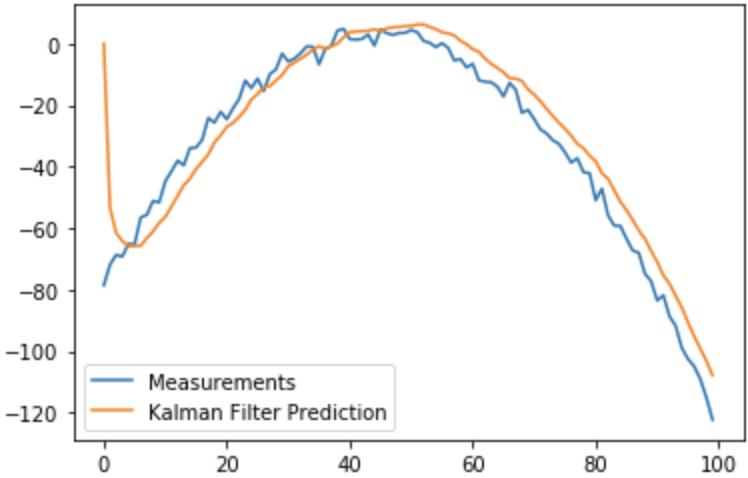
\includegraphics[width=15cm, height=10cm]{I.png}

\section*{part J}
\begin{problem}
  \problemquestion{using KF function implement LQG controller}
\end{problem}

\begin{lstlisting}
M = 1000;
m1 = 100;
m2 = 100;
l1 = 20;
l2 = 10;
g = 9.80;
x0= [ 5 ; 0 ; 0.1 ; 0 ;0.2 ; 0 ; 0 ; 0 ; 0 ; 0 ; 0 ; 0]
A= [0 1 0 0 0 0 ; 0 0 -(m1*g/M) 0 -(m2*g/M) 0 ; 0 0 0 1 0 0 ; 0 0 -(g*(M+m1))/(M*l1) 0 -(m2*g)/(M*l1) 0 ;0 0 0 0 0 1; 0 0 -(m1*g)/(M*l2) 0 -(g*(M+m2))/(M*l2) 0]
B= [ 0; 1/M ;0; 1/(M*l1) ;0 ;1/(M*l2)];
C = [1 0 0 0 0 0];
D = 0;
Q=[1 0 0 0 0 0;0 1 0 0 0 0; 0 0 100 0 0 0; 0 0 0 1000 0 0; 0 0 0 0 150 0; 0 0 0 0 0 1500]
R=0.0001
K = lqr(A,B,Q,R);
sys_1 = ss(A,[B B],C,[zeros(1,1) zeros(1,1)]);
vd = 0.3;
vn = 1;
sen = [1];
known = [1];
[~,L,~] = kalman(sys_1,vd,vn,[],sen,known)
Ac = [A-B*K B*K;zeros(size(A)) A-L*C];
Bc = zeros(12,1);
Cc = [C zeros(size(C))];
sys_cl_lqg = ss(Ac,Bc,Cc,D );

t = 0:0.01:100;
F = zeros(size(t));
[Y,~,X] = lsim(sys_cl_lqg,F,t,x0);
figure
plot(t,Y(:,1),'b');
u = zeros(size(t));
for i = 1:size(X,1)
u(i) = K * (X(i,1:6))';
end
Xhat = X(:,1) - X(:,6);
figure(2);
hold on
plot(t,Xhat)

plot(t,X(:,1),'r')
legend('X__hat','X')
hold off



x0 =

    5.0000
         0
    0.1000
         0
    0.2000
         0
         0
         0
         0
         0
         0
         0


A =

         0    1.0000         0         0         0         0
         0         0   -0.9800         0   -0.9800         0
         0         0         0    1.0000         0         0
         0         0   -0.5390         0   -0.0490         0
         0         0         0         0         0    1.0000
         0         0   -0.0980         0   -1.0780         0


Q =

           1           0           0           0           0           0
           0           1           0           0           0           0
           0           0         100           0           0           0
           0           0           0        1000           0           0
           0           0           0           0         150           0
           0           0           0           0           0        1500


R =

   1.0000e-04


L =

    0.0303
    0.0005
    0.0000
    0.0000
    0.0001
    0.0000

\end{lstlisting}{}

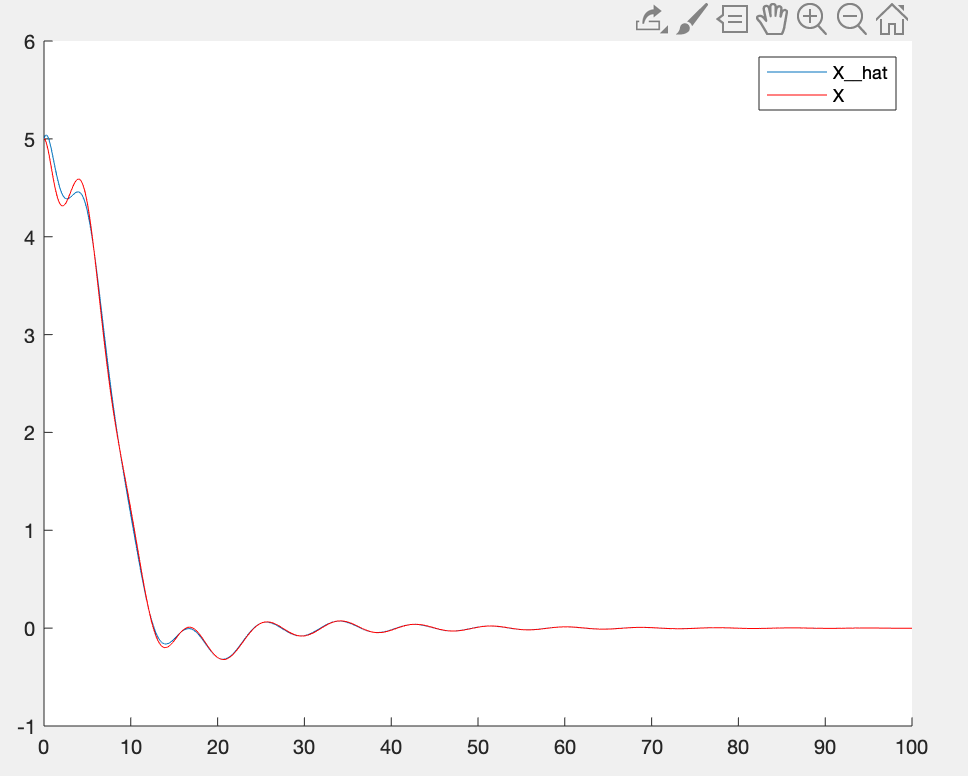
\includegraphics[width=15cm, height=10cm]{J.png}


\end{document}
